\documentclass[dvipdfmx]{jsarticle}
\usepackage[T1]{fontenc}
\usepackage[dvipdfmx]{hyperref}
\usepackage{lmodern}
\usepackage{latexsym}
\usepackage{amsfonts}
\usepackage{amssymb}
\usepackage{mathtools}
\usepackage{nccmath}
\usepackage{amsthm}
\usepackage{multirow}
\usepackage[dvipdfmx]{graphicx}
\usepackage{wrapfig}
\usepackage{here}
\usepackage{float}
\usepackage{ascmac}
\usepackage{url}

\def\NO{02}
\def\LECTURENAME{論理と計算}
\begin{document}
\title{\LECTURENAME{}:第\NO{}回演習問題}

\author{5419045 高林秀}

\date{}
\maketitle

\begin{itemize}
\item Latexを用いて作成し,PDF形式で提出してください
\end{itemize}


\vspace*{\baselineskip}

\begin{enumerate}\setlength{\itemsep}{\baselineskip}
\item 以下の(括弧が省略された)各複合文に対し,括弧を省略しない表記を示した上で,
  それが否定文,連言文,選言文,含意文,同値文のいずれであるか回答しなさい.

  \begin{enumerate}
  \item $p \land q \land r \lor s$

  \item $p\Leftrightarrow q\lor r$

  \item $\neg p \lor q \land r \Rightarrow s$

  \end{enumerate}
  \paragraph{解答}
  \begin{enumerate}
    \item $(p \wedge q \wedge r) \vee (s)$:選言文
    \item $(p) \Leftrightarrow (q \vee r)$:同値文
    \item $((\ulcorner p \vee q) \wedge r) \Rightarrow (s)$:含意文
  \end{enumerate}


\item 以下の各文同士が等価であるか否かを,真理値表を用いて示しなさい(真理値表を書きましょう).
  \begin{enumerate}
  \item
    命題文$\alpha\Leftrightarrow\beta$と
    命題文$(\alpha\Rightarrow\beta)\land (\beta\Rightarrow\alpha)$

  \item
    命題文$\alpha\Leftrightarrow\beta$と
    命題文
    $\neg((\alpha\Rightarrow\beta)\Rightarrow\neg(\beta\Rightarrow\alpha))$

  \item
    命題文$\alpha\Leftrightarrow\beta$と
    命題文
    $\neg( \neg(\neg\alpha\lor\beta)\lor\neg(\neg\beta\lor\alpha) )$
  \end{enumerate}
  \paragraph{解答}
  \begin{enumerate}
    \item 等価
    \item 等価
    \item 等価
  \end{enumerate}
  真理値表は下図
  \begin{figure}[H]
    \centering
    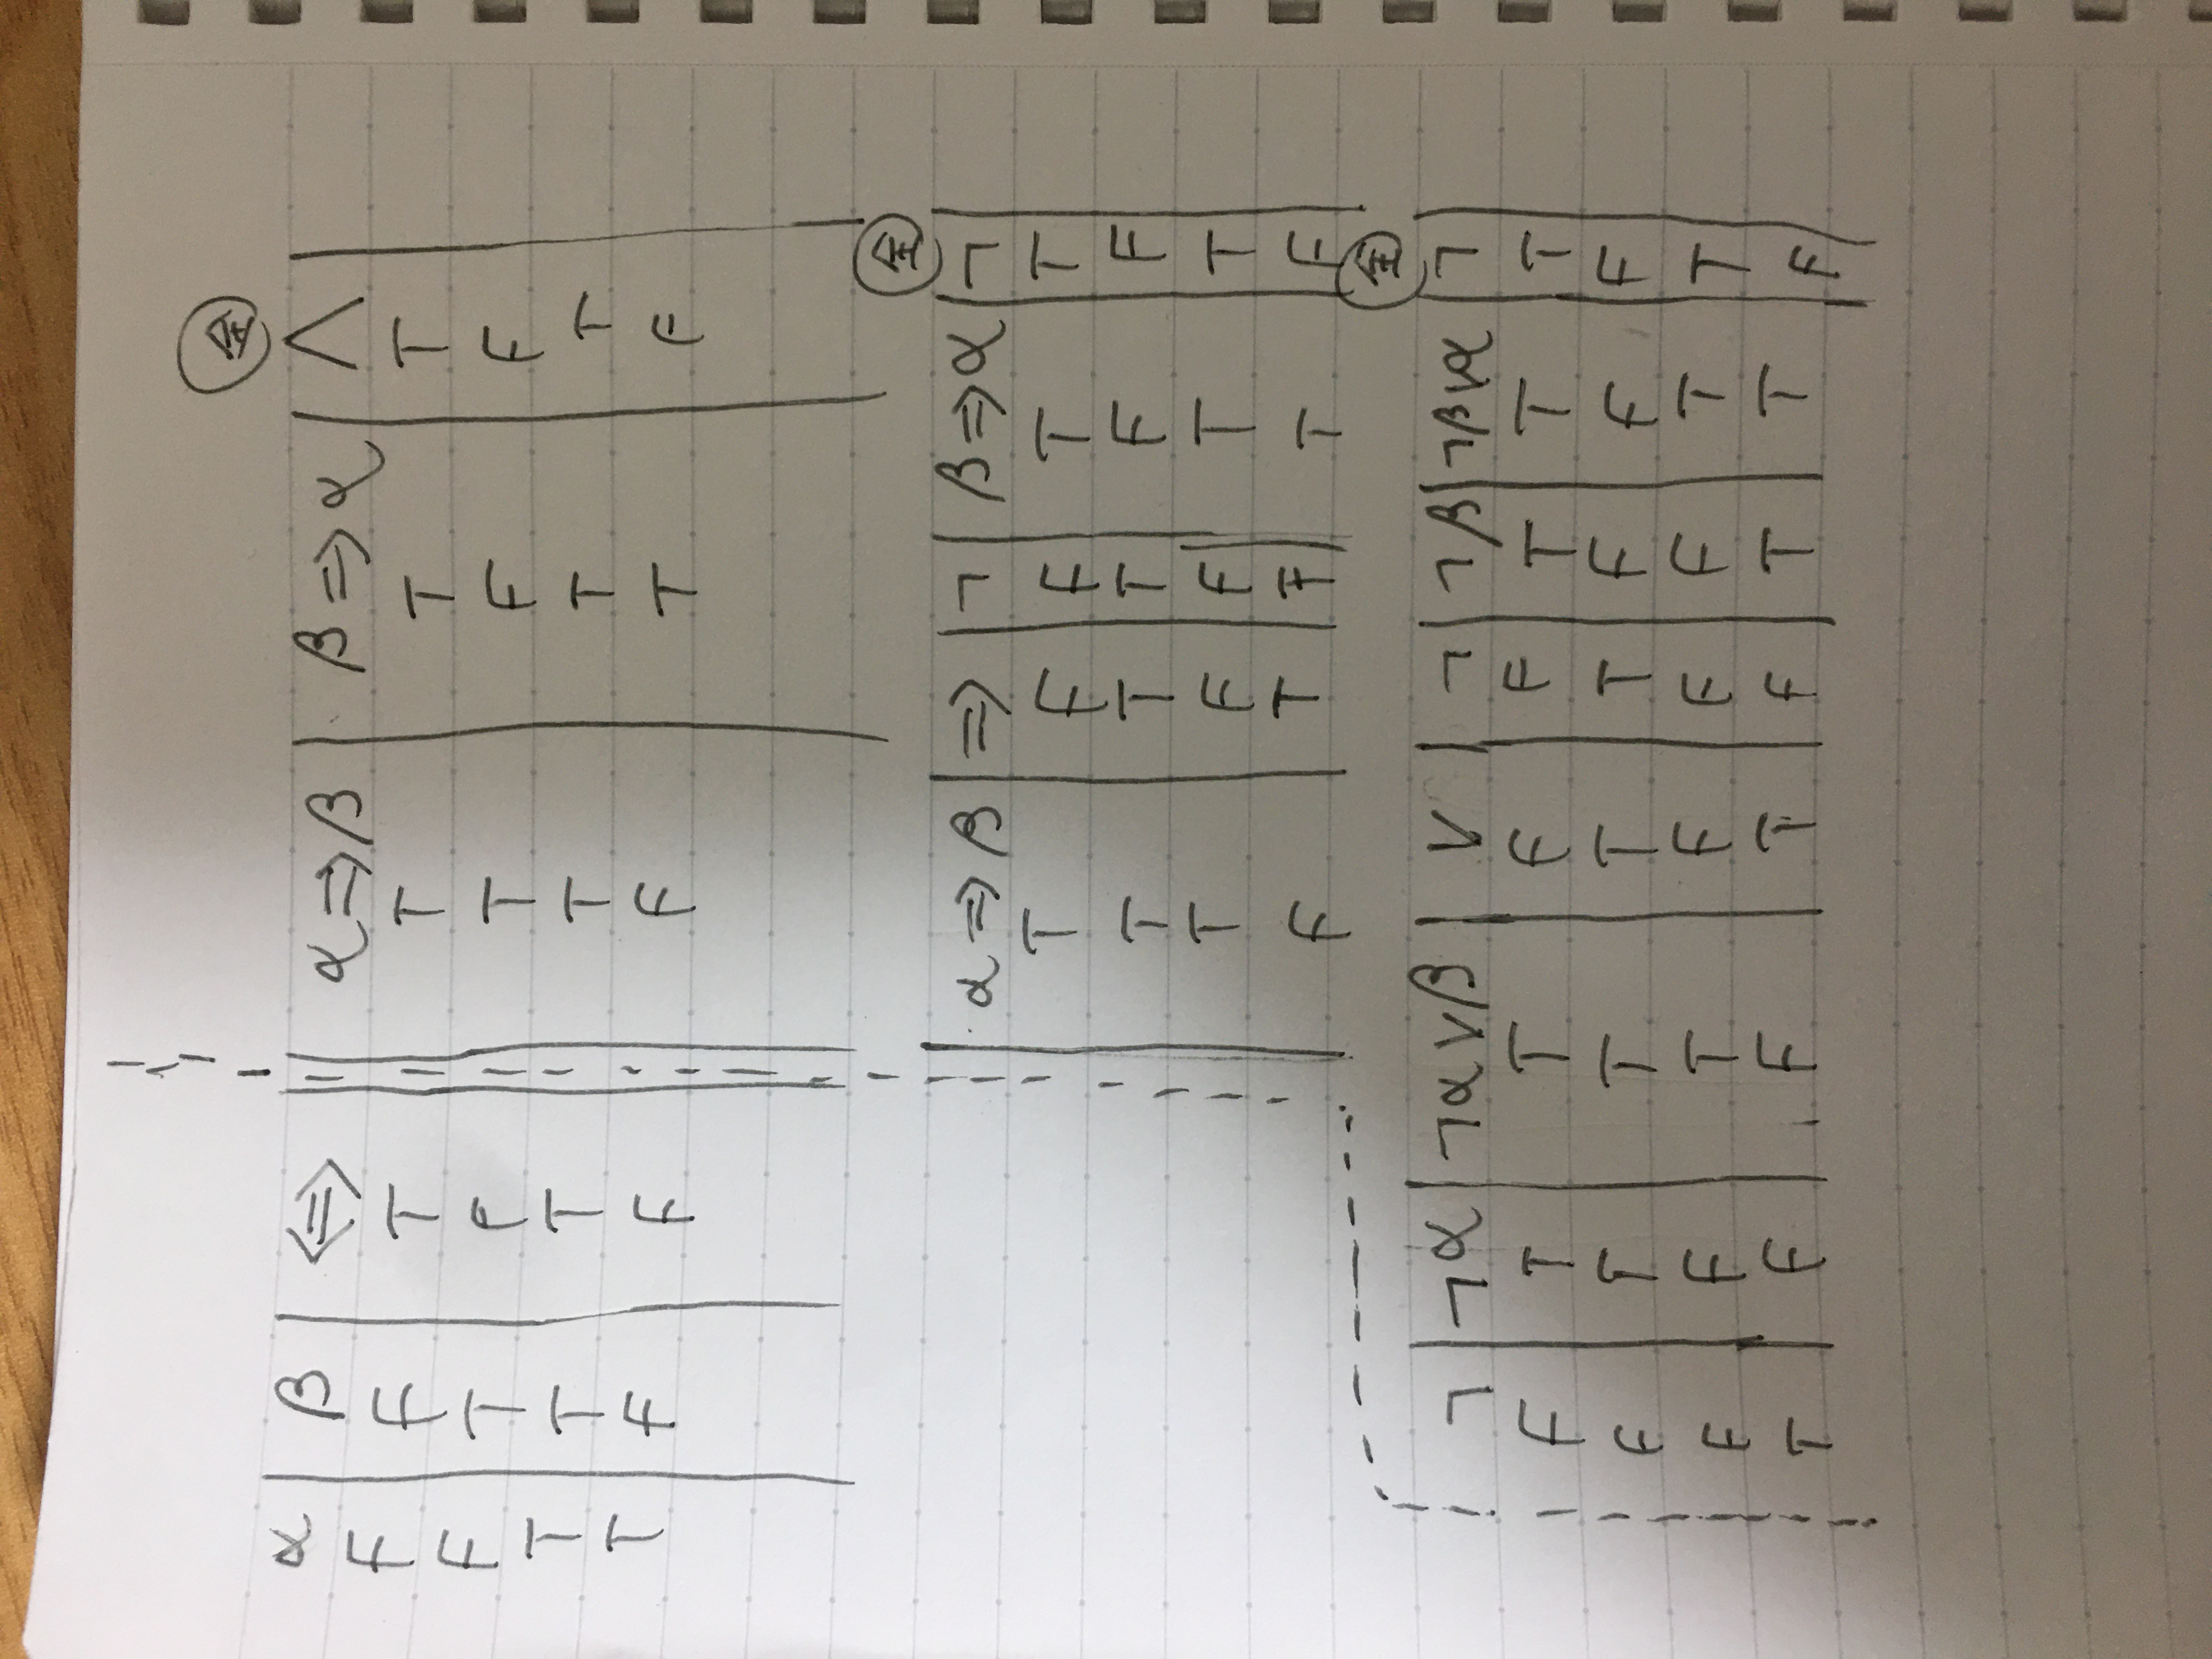
\includegraphics[scale=0.1]{IMG_4934.JPG}
  \end{figure}


\item
  $(p\lor(\neg q\land r))\Rightarrow s$を選言標準形に変換しなさい(変形の過程を示すこと).



\item
  講義資料におけるWumpus Worldの知識ベース
  $R1 \land R2 \land R3 \land R4 \land R5$のモデルを求め,
  [1,1], [1,2], [2,1], [2,2], [3,1]の各部屋に,
  穴があるか・ないか・判断不能かを示しなさい.

  ※モデルとは,知識ベースを真にする解釈(真理値の割り当て)です.
  今回,命題変数の数は7ですので,解釈の総数は$2^7=128$となります.
  (何の考えもなしの)手作業だとかなりつらいです.
  手順を考えるか,プログラミングを用いて求めることが望まれます.


\end{enumerate}
\end{document}
